\subsection{Lifetime, Delivery and Energy}
Table~\ref{tab:life} and Fig.~\ref{fig:alive} give the lossy-channel results. QHP-Net's first death comes at round $2{,}133\pm19$: 249 rounds (13.2\%) after NSGA-II, 43--52\% after the fuzzy, DQN and HIECF selectors, and 2.0$\times$ after LEACH. Its FND standard deviation is 0.58 of NSGA-II's and one fifteenth of PEGASIS's. Only TEEN dies later, and only because it suppresses 89\% of the readings.

QHP-Net delivers 98.3\% of the readings it senses, the highest yield of any clustered protocol, and spends 0.470\,mJ per delivered reading, 16\% less than the cheapest baseline (PEGASIS and NSGA-II, 0.56\,mJ). It lives longer \emph{and} delivers more data per joule, which is the green-network result. Retransmissions take 0.2\% of its budget, against 3.6\% for NSGA-II and 5.3\% for LEACH, because the learned ETX keeps sink hops out of the packet-error waterfall. This holds although it pays the largest control share of the centralised protocols (5.3\%).

Max--min balancing has a cost. Nodes run down together, so HND follows FND by only 32 rounds and the last node dies at round 2,208, before NSGA-II (2,397), DQN (2,477), PEGASIS (2,560) and Direct (3,186). For coverage, keeping every node alive to round 2,133 is worth more than keeping a few to round 2,500. On the area under the alive curve, which counts both, QHP-Net ties PEGASIS ($216.4$ vs.\ $216.2\times10^3$, n.s.) and beats every other full-yield protocol, NSGA-II by $15.4\times10^3$.

\emph{Upper bound.} Until the first death every reading must leave its node each round, costing at least one transmission plus either the sink amplifier or a reception and fusion elsewhere. Summing this floor, with no control, retries or relaying, bounds FND at \fndbound{} rounds on average; QHP-Net reaches \fndfrac\% of it.

\begin{table}[t]
\caption{Lifetime on the lossy channel, mean $\pm$ s.d.\ over 30 paired runs. AUC in $10^3$ node-rounds; mJ per delivered reading. $^c$\,censored at the 7000-round cap in every run.}
\label{tab:life}
\centering\footnotesize
\setlength{\tabcolsep}{2.6pt}
\begin{tabular}{@{}lrrrrrr@{}}
\toprule
Protocol & FND & HND & LND & AUC & Yield & mJ/rd\\
\midrule
Direct & 115 $\pm$ 10 & 1,140 $\pm$ 200 & 3,186 $\pm$ 83 & 132.6 & 0.967 & 0.78 \\
LEACH & 1,051 $\pm$ 51 & 1,674 $\pm$ 28 & 2,160 $\pm$ 43 & 166.4 & 0.867 & 0.69 \\
PEGASIS & 1,600 $\pm$ 286 & 2,202 $\pm$ 9 & 2,560 $\pm$ 290 & 216.2 & 0.827 & 0.56 \\
TEEN & 2,297 $\pm$ 145 & 5,975 $\pm$ 223 & $>$7,000$^c$ & 558.9 & 0.107 & 1.65 \\
NSGA-II & 1,884 $\pm$ 33 & 1,984 $\pm$ 28 & 2,397 $\pm$ 151 & 201.1 & 0.888 & 0.56 \\
Fuzzy-T2 & 1,476 $\pm$ 61 & 1,922 $\pm$ 28 & 2,208 $\pm$ 52 & 189.2 & 0.899 & 0.59 \\
DQN & 1,403 $\pm$ 52 & 1,875 $\pm$ 31 & 2,477 $\pm$ 79 & 189.0 & 0.882 & 0.60 \\
HIECF & 1,490 $\pm$ 128 & 1,930 $\pm$ 44 & 2,218 $\pm$ 66 & 191.2 & 0.905 & 0.58 \\
\textbf{QHP-Net} & 2,133 $\pm$ 19 & 2,165 $\pm$ 17 & 2,208 $\pm$ 27 & 216.4 & 0.983 & 0.47 \\

\bottomrule
\end{tabular}
\end{table}

\begin{figure*}[t]
\centering
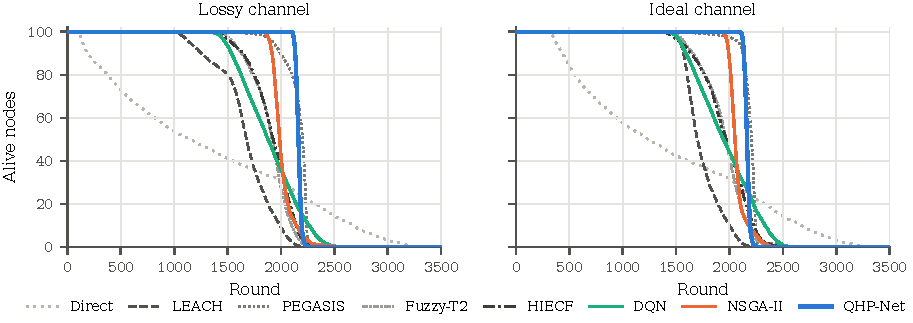
\includegraphics[width=0.94\textwidth]{alive}
\caption{Alive nodes per round, mean of 30 paired topologies (TEEN, censored at 7000 rounds, is omitted). QHP-Net keeps all 100 nodes alive longest under both channel models, and its curve does not move when packet loss is removed.}
\label{fig:alive}
\end{figure*}

\subsection{Paired $t$-Tests}
Table~\ref{tab:ttest} tests the per-topology differences. QHP-Net's first death is later than that of every full-yield opponent in \emph{all} 30 topologies on both channels; its smallest single margin over NSGA-II is 198 rounds (lossy) and 137 (ideal). Against NSGA-II the mean FND gain is $+249$ rounds, 95\% CI $[+238,+260]$, $t(29)=46.2$, $p_{Holm}=4.3\times10^{-28}$, $d_z=8.4$. The AUC gain is $15.4\times10^3$ node-rounds ($t(29)=38.0$, $d_z=6.9$). Shapiro--Wilk does not reject normality for NSGA-II ($p{=}0.23$) but does for some pairs (PEGASIS FND, $p{=}0.001$), so every cell was confirmed with the Wilcoxon test. All cells but one are significant under both tests after Holm correction ($p\le1.0\times10^{-5}$).

In our earlier study the FND gains of the fuzzy and DQN selectors over LEACH (417 and 426 rounds) shrank to an insignificant 17 and 22 on an ideal channel~\cite{sharma2026unified}. QHP-Net's gain does not vanish: without loss it still leads NSGA-II by 168 rounds ($d_z=8.6$) and every other full-yield protocol by 478--1,806. Its own FND is 2,133 on both channels, so its advantage comes from where energy is drawn, not only from avoiding loss. PEGASIS is the one opponent it does not beat on every metric: they tie on AUC under loss, and PEGASIS leads by $2.7\times10^3$ node-rounds on the ideal channel and reaches HND 37 rounds later. In exchange QHP-Net delivers 15.6 points more readings and its first node dies 533 rounds later.

\begin{table*}[t]
\caption{Paired differences QHP-Net $-$ opponent over 30 topologies: mean [95\% CI] and Cohen's $d_z$. Unless marked $^{ns}$, the difference is significant under both the paired $t$-test and the Wilcoxon test after Holm correction across opponents ($p\le1.0\times10^{-5}$). AUC in $10^3$ node-rounds. TEEN reaches its lead by delivering 11\% of the readings.}
\label{tab:ttest}
\centering\footnotesize
\begin{tabular}{@{}lrrrrrrrr@{}}
\toprule
& \multicolumn{2}{c}{$\Delta$FND, lossy} & \multicolumn{2}{c}{$\Delta$FND, ideal} & \multicolumn{2}{c}{$\Delta$AUC, lossy} & \multicolumn{2}{c}{$\Delta$AUC, ideal}\\
\cmidrule(lr){2-3}\cmidrule(lr){4-5}\cmidrule(lr){6-7}\cmidrule(l){8-9}
Opponent & mean [95\% CI] & $d_z$ & mean [95\% CI] & $d_z$ & mean & $d_z$ & mean & $d_z$\\
\midrule
LEACH & +1,082 [+1,062, +1,101] & 20.8 & +652 [+641, +662] & 23.0 & +50.0 & 19.9 & +42.2 & 24.9 \\
PEGASIS & +533 [+425, +641] & 1.8 & +478 [+362, +594] & 1.5 & +0.3$^{ns}$ & 0.1 & -2.7 & -1.4 \\
TEEN & -164 [-216, -111] & -1.2 & -2,154 [-2,207, -2,100] & -15.1 & -342.5 & -25.0 & -376.8 & -42.5 \\
NSGA-II & +249 [+238, +260] & 8.4 & +168 [+161, +175] & 8.6 & +15.4 & 6.9 & +9.5 & 6.6 \\
Fuzzy-T2 & +658 [+634, +682] & 10.3 & +632 [+609, +655] & 10.2 & +27.2 & 10.2 & +22.3 & 9.6 \\
DQN & +730 [+710, +750] & 13.6 & +657 [+648, +666] & 26.8 & +27.5 & 10.9 & +20.9 & 12.2 \\
HIECF & +643 [+595, +692] & 5.0 & +648 [+606, +690] & 5.7 & +25.3 & 8.3 & +21.0 & 7.9 \\

\bottomrule
\end{tabular}
\end{table*}



